 \documentclass[a4paper,11pt]{article}
 \usepackage{latexsym}
 \usepackage[utf8]{inputenc}
 \usepackage[activeacute,spanish]{babel}
 \RequirePackage{graphicx}
 \RequirePackage{booktabs}
 \title{REPORTE: ESTIMACIÓN DE PARÁMETROS DE TSUNAMI DE ORIGEN LEJANO}
 \author{Cesar Jimenez \\
 (Version: 1.3)}
 \frenchspacing
 \begin{document}
 \renewcommand{\tablename}{Tabla}
 \maketitle
 \section*{Introducción}
 \noindent
 Este reporte preliminar de tsunami de origen lejano ha sido 
 elaborado en forma automática por el modelo numérico TSDHN-2022.
 Las dimensiones de la fuente sísmica se calculan a partir de las ecuaciones de
  Papazachos et al. (2004).
 El mecanismo focal del terremoto se toma de la base de datos del Global CMT.
 El campo de deformación se obtiene a partir de las ecuaciones analíticas de
  Okada (1992).
  
 La simulación de la propagación del tsunami se realiza con el modelo 
 numérico TUNAMI, modelo lineal y en coordenadas esféricas (Imamura et al.,
  2006). La grilla batimétrica computacional abarca todo el Océano Pacífico, 
 con una resolución de 4 min o 240 s. El cálculo de las isócronas de 
 tiempos de arribo para todo el Océano Pacífico se realizó con el modelo 
 Tsunami Travel Time (Wessel, 2009).
  
 Se han colocado 3 mareógrafos virtuales en los puertos de Talara, Callao y 
 Matarani. Se utilizó la ley de Green para la corrección de la amplitud de 
 los mareogramas, debido a que los nodos computacionales no coinciden 
 necesariamente con la ubicación de las estaciones mareográficas costeras 
 (Satake, 2015).
  
 El tiempo promedio de cómputo para una PC i7 es de 15 min para una ventana 
 de tiempo de simulación de 28 horas (Figura 1). Sin embargo, el 
 supercomputador DHN demora menos de 2 minutos. \\
  
 \noindent \textbf{Nota:} El resultado del modelo TSDHN-2022 es una estimación 
 referencial y de preferencia debe ser utilizado para
 obtener los parámetros de tsunamis de origen lejano, es decir fuera de las fro
 nteras del litoral de Perú.
 Para eventos de origen cercano, se debe utilizar el modelo Pre-Tsunami (Jimenez
  et al., 2018).
 \begin{table*}
 \centerline{
 \begin{tabular}[t]{lp{0.5cm}l}
 \toprule
 Parámetro   & & Valor \\
 \midrule
Latitud     & &   56.00$^\circ$  \\
Longitud    & & -156.00$^\circ$  \\
Profundidad & &   12.0 km       \\
Magnitud    & &    9.0 Mw       \\
 \midrule
Strike      & &  247.0$^\circ$  \\
Dip         & &    8.0$^\circ$  \\
Rake        & &   90.0$^\circ$  \\
 \bottomrule
 \end{tabular}}
 \caption{Parámetros hipocentrales y mecanismo focal del terremoto.}
 \end{table*}
 \begin{figure}
 \centerline{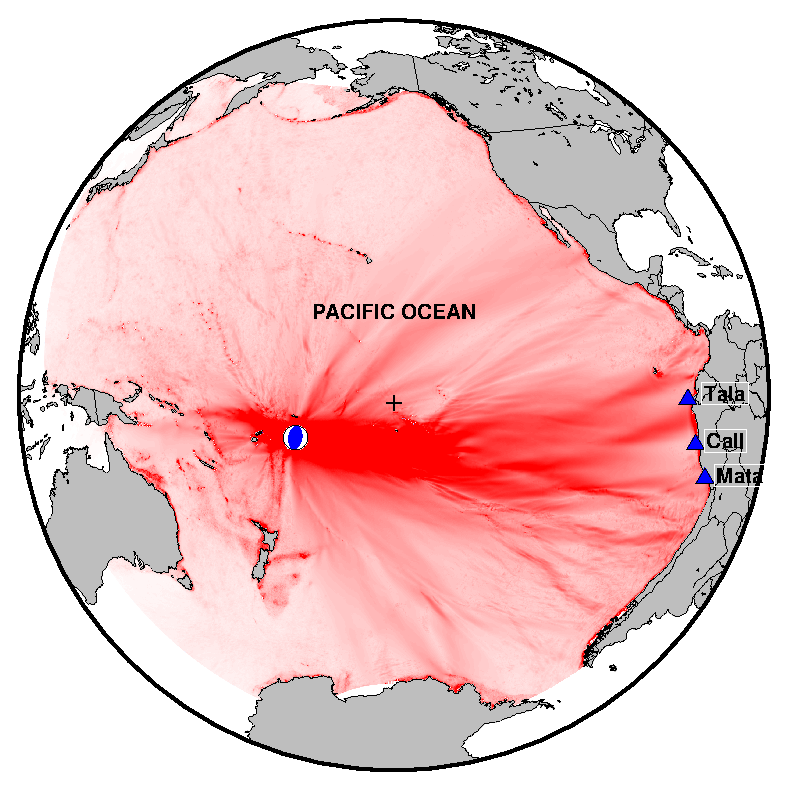
\includegraphics[scale=0.88]{maxola.eps}}
 \caption{Mapa de máxima altura de propagación del tsunami. La esfera
 focal representa el epicentro. Los triángulos azules representan 
 a las estaciones mareográficas.}
 \label{max_ola}
 \end{figure}
 \section*{Análisis}
 La Tabla 1 muestra los parámetros hipocentrales y el mecanismo focal del 
 terremoto. La Figura 1 muestra el mapa de propagacion de la máxima energía,
 la ubicación del epicentro está representado por la esfera focal y las 
 estaciones mareográficas están representadas por los triángulos azules
  
 La Figura 2 muestra las isócronas de los tiempos de arribo del tsunami para 
 todo el Oceano Pacifico. La Figura 3 muestra los mareogramas simulados para 
 las estaciones del litoral del Perú, de norte a sur: Talara, Callao y 
 Matarani. La Tabla 2 muestra los valores de los tiempos de arribo y la 
 máxima altura del tsunami en las estaciones mareográficas del litoral 
 Peruano.
 \begin{figure}
 \centerline{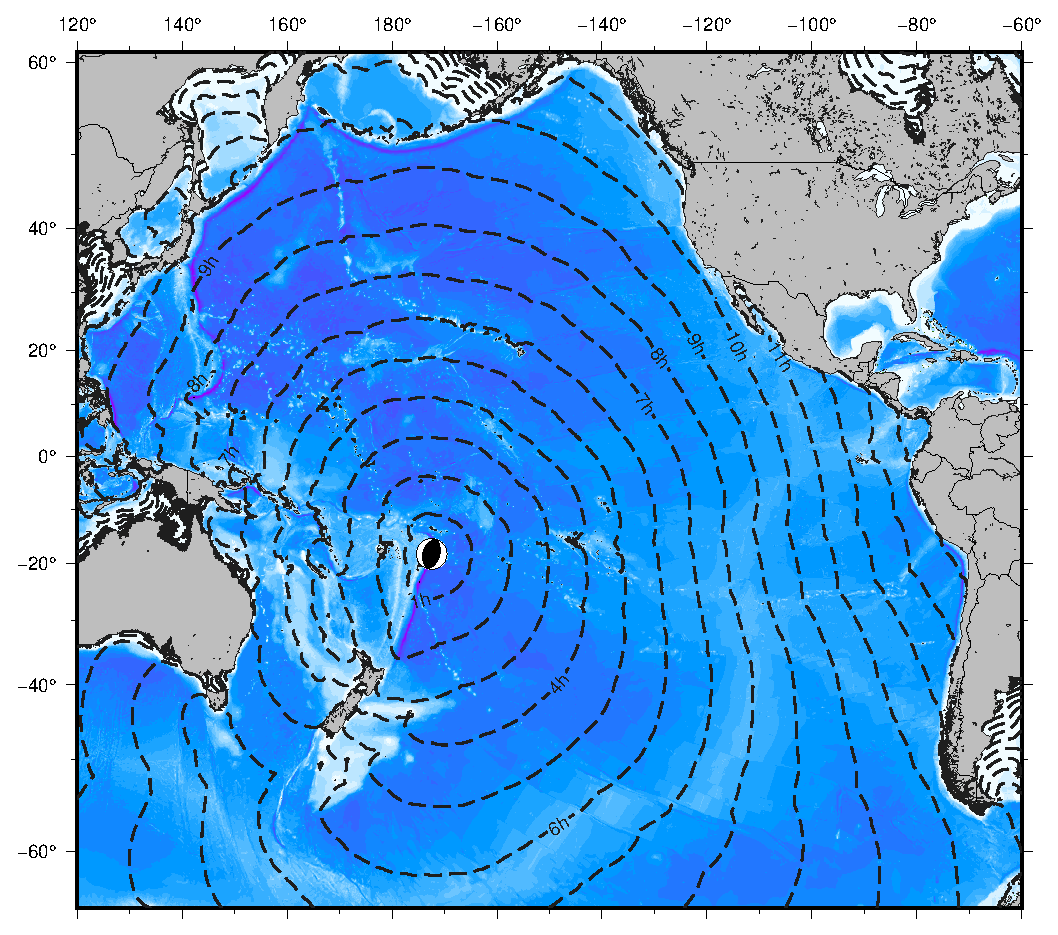
\includegraphics[scale=0.78]{ttt.eps}}
 \caption{Mapa de tiempo de arribo del tsunami. La esfera focal representa el 
 epicentro.}
 \label{ttt}
 \end{figure}
 \begin{figure}
 \centerline{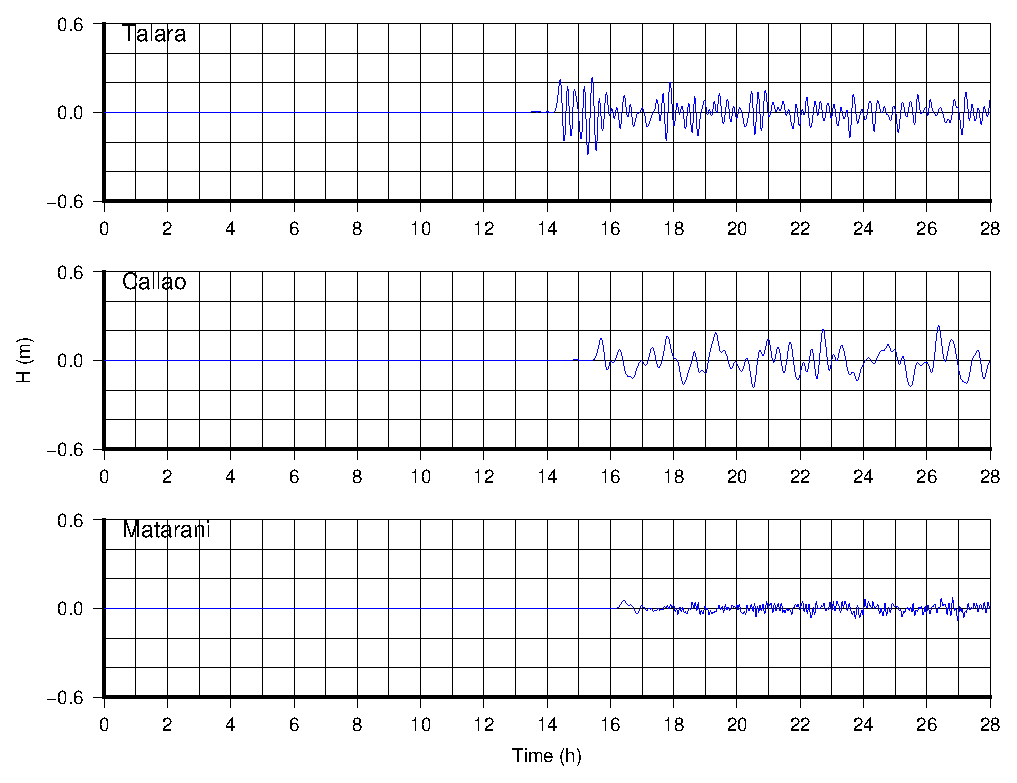
\includegraphics[scale=0.84]{mareograma.eps}}
 \caption{Mareogramas simulados en las estaciones de Talara, Callao y Matarani.}
 \end{figure}
 \begin{table*}
 \centerline{
 \begin{tabular}[t]{lcc}
 \toprule
 Estación     & Tiempo de arribo & Máximo (m) \\
 \midrule
Talara     &13:29 &   0.24  \\
Callao     &14:46 &   0.24  \\
Matarani   &15:29 &   0.07  \\
 \bottomrule
 \end{tabular}}
 \caption{Tiempo de arribo (hh:mm) y máxima amplitud del tsunami.}
 \end{table*}
 \begin{thebibliography}{99}
 \bibitem{1} B. Papazachos, E. Scordilis, C. Panagiotopoulus and G. Karakaisis. 
 Global relations between seismic
 fault parameters and moment magnitude of earthquakes. Bulletin of Geological 
 Society of Greece, vol XXXVI, pp 1482-1489 (2004).
 \bibitem{2} Y. Okada. Internal deformation in a half space. Bull. Seismol. Soc.
 Am. {82}(2) 1018-1040 (1992).
 \bibitem{3} F. Imamura, A. Yalciner and G. Ozyurt. Tsunami Modelling Manual
 (TUNAMI model). Tohoku University, Sendai. (2006).
 \bibitem{4} P. Wessel. Analysis of observed and predicted tsunami travel times 
 for the Pacific and Indian Oceans. Pure Appl. Geophys., vol 166, pp 301--324 (2
 009).
 \bibitem{5} K. Satake. Tsunamis, inverse problem of. Encyclopedia of Complexity
  and Systems Science, pp 1--20 (2015).
 \bibitem{6} C. Jimenez, C. Carbonel and J. Rojas. Numerical procedure to foreca
 st the tsunami parameters from a
 database of pre-simulated seismic unit sources. Pure Appl. Geophys., vol 175, p
 p 1473--1483 (2018).
 \end{thebibliography}
 \end{document}
